% !TeX program = xelatex
\documentclass[aspectratio=169,11pt]{beamer}
\usepackage{../shared/style/ghim-beamer}

\title{Energy Module: Modeling Proposal}
\author{Hyuntae Choi\inst{1}}
\institute{\inst{1} Moon Soul Graduate School of Future Strategy, KAIST}
\date{3rd March, 2026}

\begin{document}

\begin{frame}[plain]
    \titlepage
\end{frame}

\begin{frame}{General Setup}

\begin{table}[ht]
\centering
\footnotesize
\renewcommand{\arraystretch}{1.5}
\begin{tabular}{@{} >{\bfseries}l p{7.5cm} c @{}}
\toprule
Time Period & \only<1>{2000--2150, 5-year timesteps}\only<2->{\textcolor{blue!70}{2000--2150, 1-year resolution}} & \only<2->{\textcolor{blue!70}{\checkmark}} \\
Region & \only<1-2>{R10}\only<3->{\textcolor{blue!70}{UN 250 countries}} & \only<3->{\textcolor{blue!70}{\checkmark}} \\
Economy & Homogeneous production function & \\
Solution  & Recursive-dynamic & \\
Technology & Relative preference logit with stock turnover & \\
Capital Dynamics & Vintage tracking with retirement and construction delays & \\
Energy System & Integrated supply, power, and hydrogen modules & \\
Trade & Global market clearing for fossil fuels & \\
\bottomrule
\end{tabular}
\end{table}

\end{frame}

\begin{frame}{Regional Classification: AR6 R10 (249 countries)}
\centering
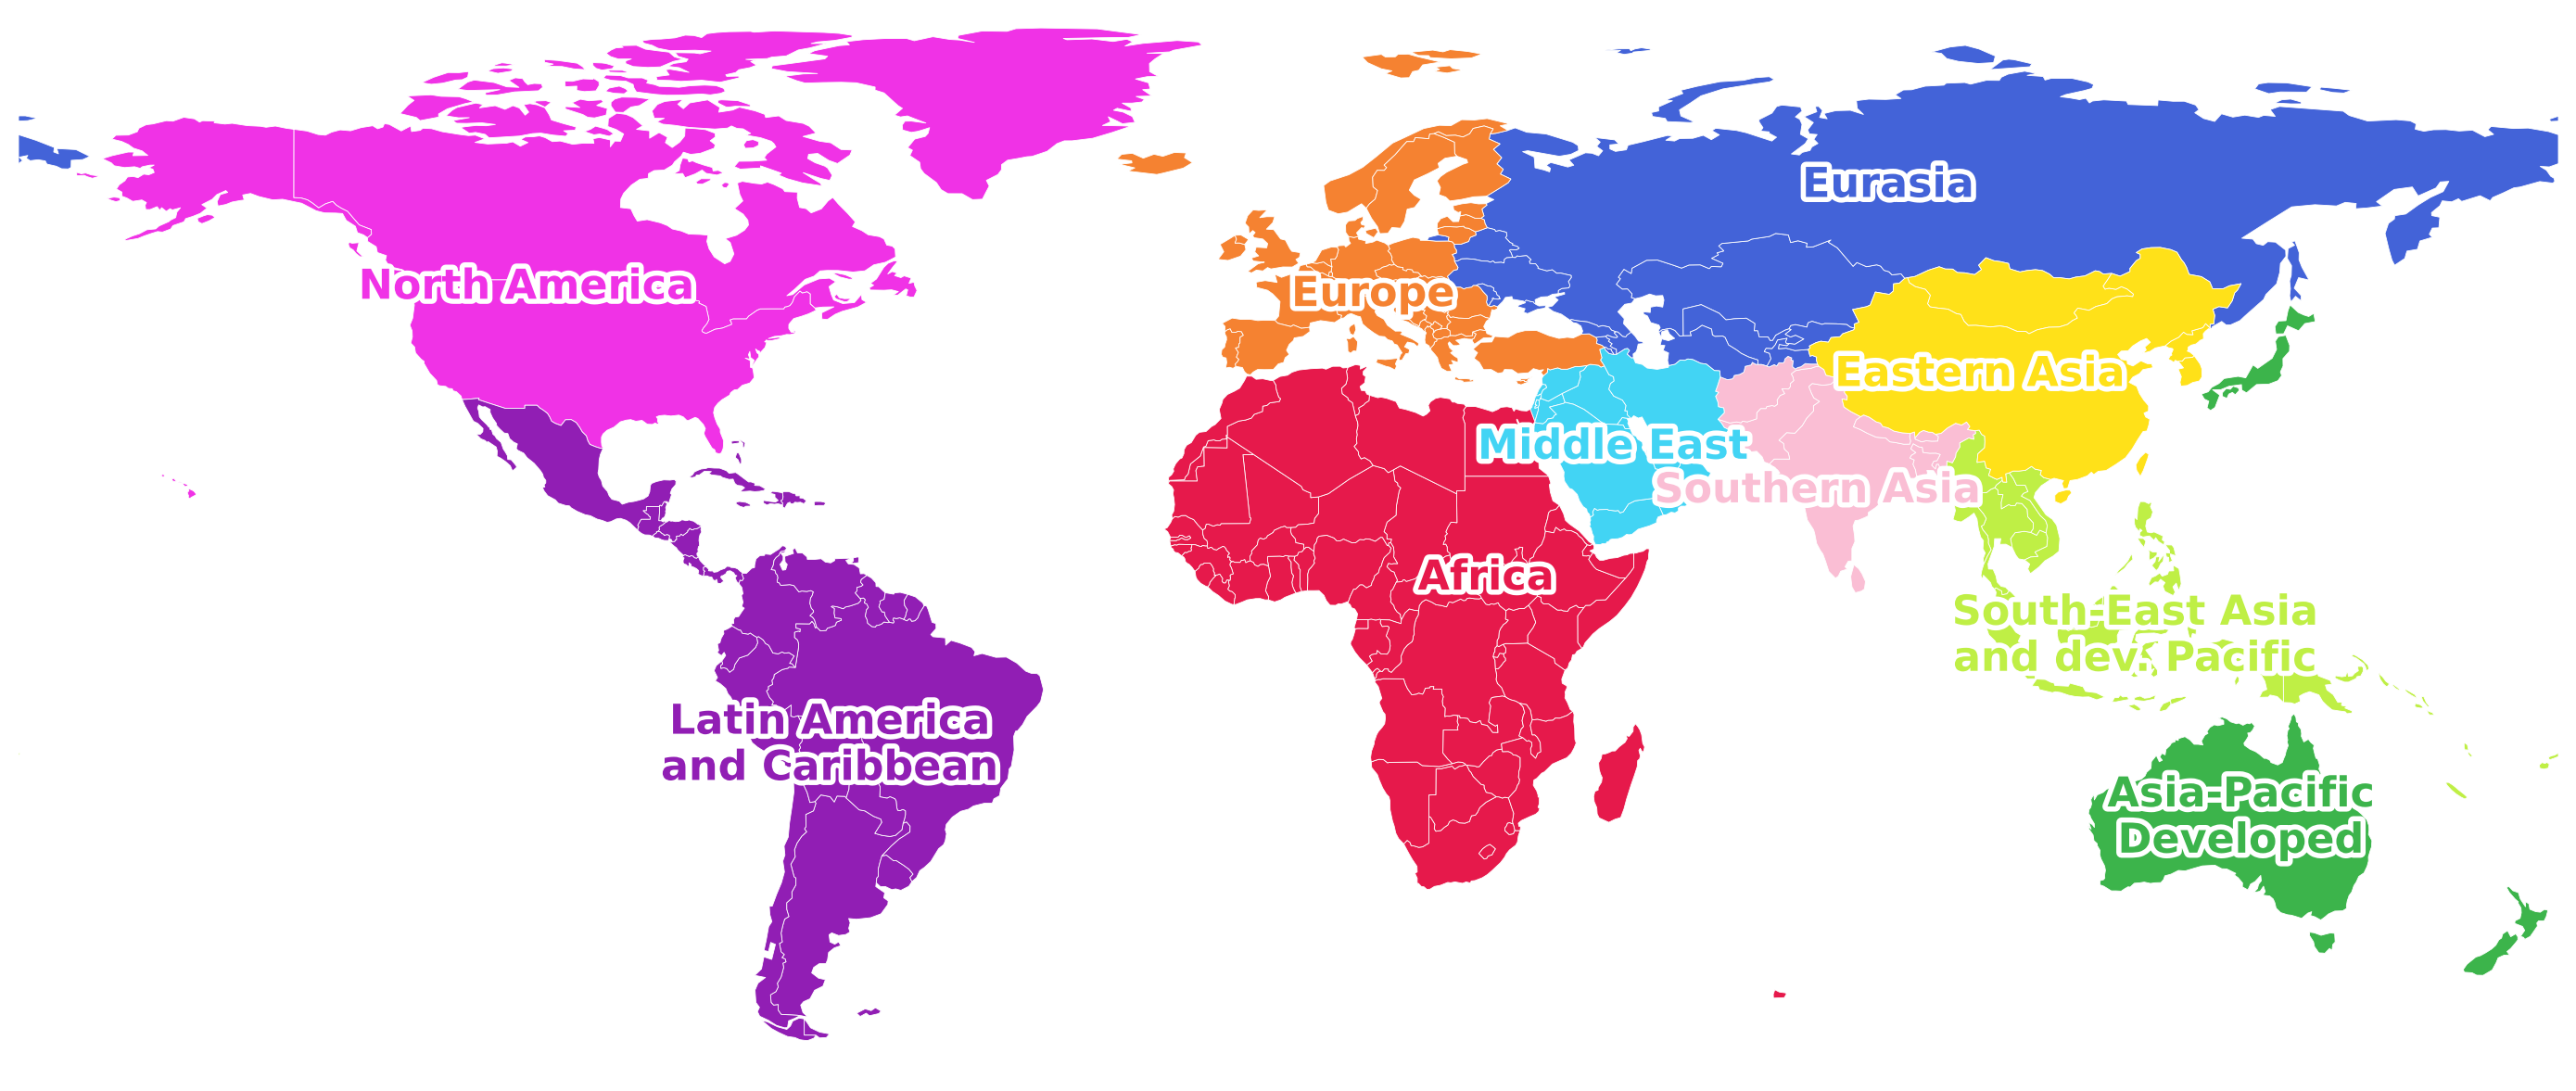
\includegraphics[width=\linewidth]{r10_world_map.png}
\end{frame}

  \begin{frame}{Model Overview}

  \centering
  \scalebox{0.85}{
  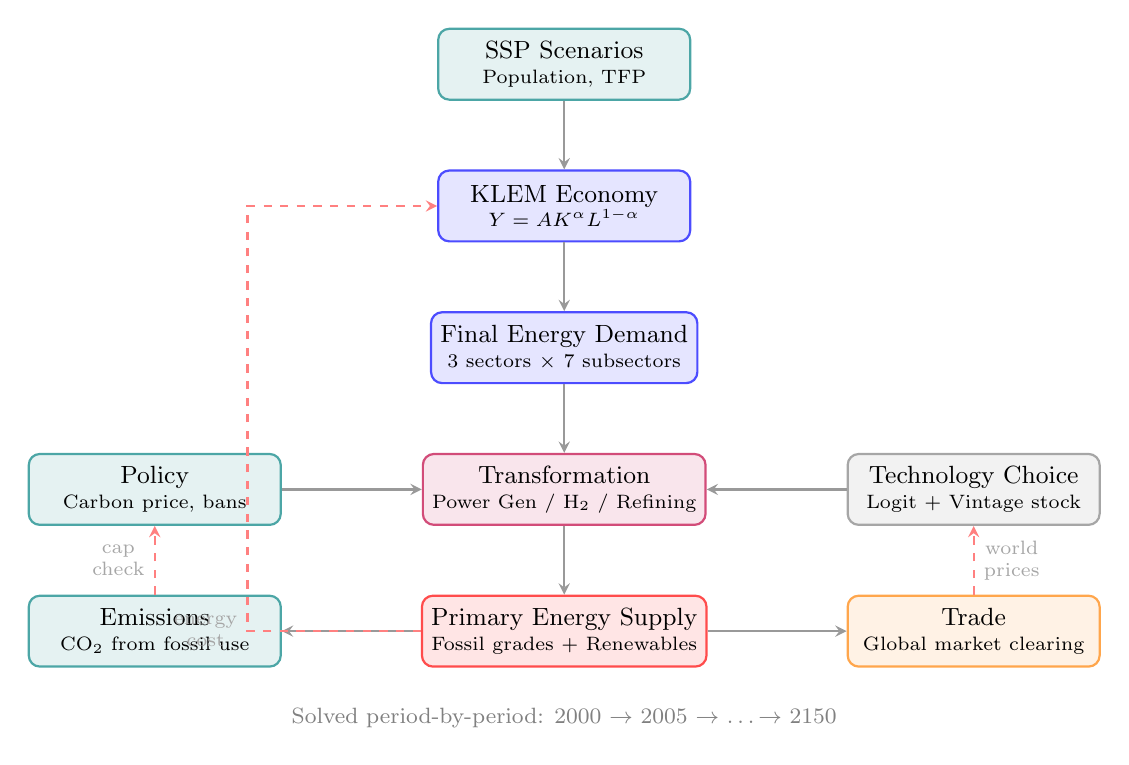
\begin{tikzpicture}[
    every node/.style={font=\small, align=center},
    boxteal/.style={rounded corners=4pt, draw=teal!70, fill=teal!10,
                minimum width=3.2cm, minimum height=0.9cm, thick},
    boxblue/.style={rounded corners=4pt, draw=blue!70, fill=blue!10,
                minimum width=3.2cm, minimum height=0.9cm, thick},
    boxpurple/.style={rounded corners=4pt, draw=purple!70, fill=purple!10,
                minimum width=3.2cm, minimum height=0.9cm, thick},
    boxred/.style={rounded corners=4pt, draw=red!70, fill=red!10,
                minimum width=3.2cm, minimum height=0.9cm, thick},
    boxorange/.style={rounded corners=4pt, draw=orange!70, fill=orange!10,
                minimum width=3.2cm, minimum height=0.9cm, thick},
    boxgray/.style={rounded corners=4pt, draw=gray!70, fill=gray!10,
                minimum width=3.2cm, minimum height=0.9cm, thick},
    arr/.style={->, >=stealth, thick, gray!80},
    fb/.style={->, >=stealth, thick, red!50, dashed},
    lbl/.style={font=\scriptsize, text=gray!70},
  ]

  % === Main vertical flow ===
  \node[boxteal]   (ssp)    at (0, 0)    {SSP Scenarios\\[-2pt]{\scriptsize Population, TFP}};
  \node[boxblue]   (klem)   at (0, -1.8) {KLEM Economy\\[-2pt]{\scriptsize $Y = AK^\alpha L^{1-\alpha}$}};
  \node[boxblue]   (demand) at (0, -3.6) {Final Energy Demand\\[-2pt]{\scriptsize 3 sectors $\times$ 7 subsectors}};
  \node[boxpurple] (trans)  at (0, -5.4) {Transformation\\[-2pt]{\scriptsize Power Gen / H$_2$ / Refining}};
  \node[boxred]    (supply) at (0, -7.2) {Primary Energy Supply\\[-2pt]{\scriptsize Fossil grades + Renewables}};

  % === Side boxes ===
  \node[boxorange] (trade)  at (5.2, -7.2) {Trade\\[-2pt]{\scriptsize Global market clearing}};
  \node[boxgray]   (tech)   at (5.2, -5.4) {Technology Choice\\[-2pt]{\scriptsize Logit + Vintage stock}};
  \node[boxteal]   (emit)   at (-5.2, -7.2) {Emissions\\[-2pt]{\scriptsize CO$_2$ from fossil use}};
  \node[boxteal]   (policy) at (-5.2, -5.4) {Policy\\[-2pt]{\scriptsize Carbon price, bans}};

  % === Main arrows ===
  \draw[arr] (ssp)    -- (klem);
  \draw[arr] (klem)   -- (demand);
  \draw[arr] (demand) -- (trans);
  \draw[arr] (trans)  -- (supply);

  % === Side arrows ===
  \draw[arr] (supply) -- (trade);
  \draw[arr] (tech)   -- (trans);
  \draw[arr] (supply) -- (emit);
  \draw[arr] (policy) -- (trans);

  % === Feedback loops ===
  \draw[fb] (supply.west) -- ++(-2.2, 0) node[lbl, left] {energy\\cost} |- (klem.west);
  \draw[fb] (trade.north) -- (tech.south) node[lbl, midway, right] {world\\prices};
  \draw[fb] (emit.north)  -- (policy.south) node[lbl, midway, left] {cap\\check};

  % === Period label ===
  \node[font=\footnotesize, text=gray] at (0, -8.3) {Solved period-by-period: 2000 $\to$ 2005 $\to$ \ldots $\to$ 2150};

  \end{tikzpicture}
  }

  \end{frame}

\begin{frame}{KLEM: Macroeconomic Core}

  \textbf{Homogeneous General Equilibrium with Energy Cost Feedback}

  \vspace{0.3em}

  \begin{columns}[T]
  \column{0.52\textwidth}

  \underline{Production \& Capital Dynamics}
  \begin{align*}
  Y_t &= A_t \cdot K_t^{\,\alpha} \cdot L_t^{\,1-\alpha} \\[4pt]
  Y_t^{\text{net}} &= Y_t - \underbrace{\textstyle\sum_c E_c \cdot p_c}_{C^{\text{energy}}} \\[4pt]
  I_t &= s \cdot Y_t^{\text{net}} \\[4pt]
  K_{t+1} &= (1-\delta)^{\Delta t} K_t + I_t \cdot \Delta t
  \end{align*}

  \vspace{0.3em}
  \underline{TFP Calibration}
  \begin{itemize}\small
    \item $A_t$ calibrated from SSP GDP path
  \end{itemize}

  \column{0.45\textwidth}

  \underline{KLEM--Sector Coupling}
  \begin{itemize}\small
    \item KLEM sets total energy envelope
    \item Sectors set relative shares
    \item Logit determines fuel mix
    \item Scale factor: $\lambda = E^{\text{KLEM}} / \sum_s E_s$
  \end{itemize}

  \vspace{0.5em}
  \begin{alertblock}{\small Capital Layer Inconsistency}
  \small
  \begin{itemize}\small
    \item $I_{\text{total}} = I_{\text{energy}} + I_{\text{non-energy}}$
    \item Capex sets price, not spending
    \item No crowding-out
  \end{itemize}
  \end{alertblock}

  \end{columns}

\end{frame}

\begin{frame}{SSP Emulation (GDP)}
\begin{center}

    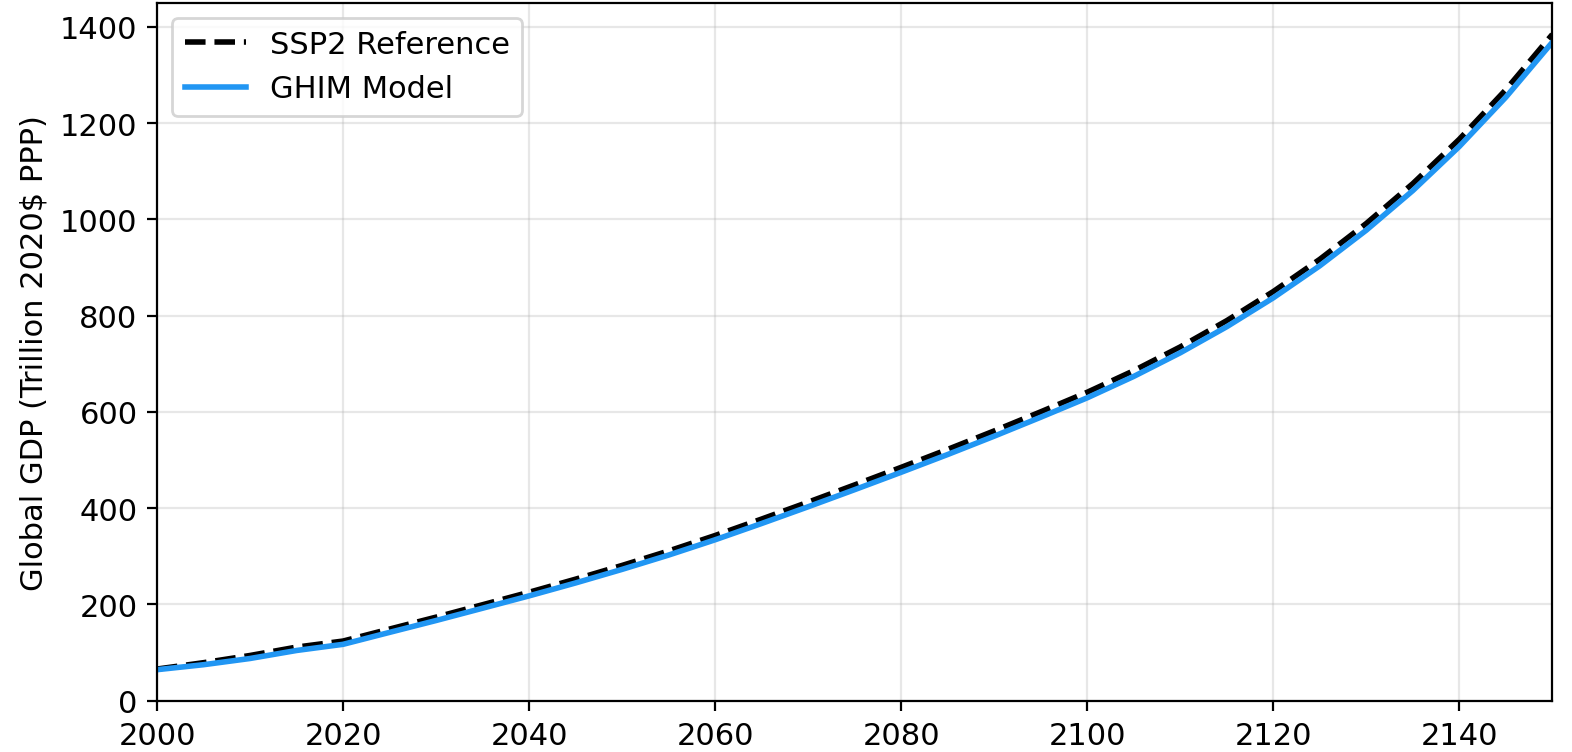
\includegraphics[width=0.85\linewidth]{gdp_trajectory.png}

\end{center}
\end{frame}

\begin{frame}{Primary Energy Demand --- Derived Demand}

  \centering
  \scalebox{0.82}{
  \begin{tikzpicture}[
    every node/.style={font=\small, align=center},
    sector/.style={rounded corners, draw=blue!70, fill=blue!10,
                   minimum width=2.2cm, minimum height=0.7cm},
    subsec/.style={rounded corners, draw=gray, fill=gray!10,
                   minimum width=1.5cm, minimum height=0.5cm, font=\scriptsize},
    carrier/.style={rounded corners, draw=orange!80, fill=orange!10,
                    minimum width=2.2cm, minimum height=0.75cm},
    fuel/.style={rounded corners, draw=red!60, fill=red!10,
                 minimum width=2.2cm, minimum height=0.75cm},
    transform/.style={rounded corners, draw=purple!70, fill=purple!10,
                      minimum width=2.6cm, minimum height=0.7cm},
    arr/.style={->, >=stealth, thick, gray!70},
    carrarr/.style={->, >=stealth, very thin, gray!70, opacity=0.55},
    darr/.style={->, >=stealth, very thick, red!60, dashed},
  ]

  % === Row 0 ===
  \node[font=\bfseries] (gdp) at (0, 0) {GDP $\;\xrightarrow\;$ Energy demand};

  % === Row 1 ===
  \node[sector] (ind) at (-5, -1.5) {Industry};
  \node[sector] (bld) at ( 0, -1.5) {Buildings};
  \node[sector] (trn) at ( 5, -1.5) {Transport};

  \draw[arr] (gdp.south) -- (ind.north);
  \draw[arr] (gdp.south) -- (bld.north);
  \draw[arr] (gdp.south) -- (trn.north);

  % === Row 2 ===
  \node[subsec] (heavy) at (-6.8, -3.1) {Heavy};
  \node[subsec] (light) at (-5.1, -3.1) {Light};
  \node[subsec] (dc)    at (-3.3, -3.1) {AI/Data};

  \node[subsec] (res) at (-1.0, -3.1) {Residential};
  \node[subsec] (com) at ( 1.0, -3.1) {Commercial};

  \node[subsec] (pass) at (4.2, -3.1) {Passenger};
  \node[subsec] (frt)  at (5.8, -3.1) {Freight};

  \draw[arr, thin] (ind.south) -- (heavy.north);
  \draw[arr, thin] (ind.south) -- (light.north);
  \draw[arr, thin] (ind.south) -- (dc.north);
  \draw[arr, thin] (bld.south) -- (res.north);
  \draw[arr, thin] (bld.south) -- (com.north);
  \draw[arr, thin] (trn.south) -- (pass.north);
  \draw[arr, thin] (trn.south) -- (frt.north);

  % === Row 3 (final energy carriers) ===
  \node[carrier] (elec) at (-2.4, -4.8) {Electricity};
  \node[carrier] (bio)  at ( 0.0, -4.8) {Biomass};
  \node[carrier] (h2)   at ( 2.4, -4.8) {Hydrogen};

  % === Row 4 (conversion) ===
  \node[transform] (pgen) at (-2.4, -5.9) {Power Gen.};
  \node[transform] (h2p)  at ( 2.4, -5.9) {H$_2$ Prod.};

  \draw[arr] (elec.south) -- (pgen.north);
  \draw[arr] (h2.south)   -- (h2p.north);

  % === Row 5 (primary fuels) ===
  \node[fuel] (coal) at (-5.0, -7.1) {Coal};
  \node[fuel] (gas)  at ( 0.0, -7.1) {Gas};
  \node[fuel] (liq)  at ( 5.0, -7.1) {Ref.\ Liquids};

  % conversion-induced fuel demand (bold red dashed)
  \draw[darr] (pgen.south west) to[bend right=10] (coal.north);
  \draw[darr] (pgen.south)      --                 (gas.north);
  \draw[darr] (h2p.south)       --                 (gas.north east);

  % === ALL subsector -> carriers/fuels (thin, semi-transparent) ===
  % Heavy
  \draw[carrarr] (heavy.south) -- (coal.north);
  \draw[carrarr] (heavy.south) -- (gas.north);
  \draw[carrarr] (heavy.south) to[bend left=10] (elec.north);
  \draw[carrarr] (heavy.south) to[bend left=8]  (liq.north west);
  \draw[carrarr] (heavy.south) to[bend right=10] (bio.north west);
  \draw[carrarr] (heavy.south) to[bend left=14] (h2.north);

  % Light
  \draw[carrarr] (light.south) -- (elec.north);
  \draw[carrarr] (light.south) -- (gas.north);
  \draw[carrarr] (light.south) to[bend left=8]  (liq.north);
  \draw[carrarr] (light.south) to[bend left=10] (coal.north east);
  \draw[carrarr] (light.south) to[bend right=10] (bio.north);
  \draw[carrarr] (light.south) to[bend left=14] (h2.north west);

  % AI/Data
  \draw[carrarr] (dc.south) -- (elec.north);

  % Residential
  \draw[carrarr] (res.south) -- (elec.north);
  \draw[carrarr] (res.south) -- (gas.north);
  \draw[carrarr] (res.south) to[bend right=10] (bio.north);
  \draw[carrarr] (res.south) to[bend left=12]  (liq.north west);
  \draw[carrarr] (res.south) to[bend left=14]  (coal.north);
  \draw[carrarr] (res.south) to[bend left=16]  (h2.north);

  % Commercial
  \draw[carrarr] (com.south) -- (elec.north);
  \draw[carrarr] (com.south) -- (gas.north);
  \draw[carrarr] (com.south) to[bend left=10] (liq.north);
  \draw[carrarr] (com.south) to[bend right=10] (bio.north east);
  \draw[carrarr] (com.south) to[bend left=14] (coal.north east);
  \draw[carrarr] (com.south) to[bend left=16] (h2.north);

  % Passenger
  \draw[carrarr] (pass.south) -- (liq.north);
  \draw[carrarr] (pass.south) to[bend right=10] (elec.north east);
  \draw[carrarr] (pass.south) to[bend right=12] (gas.north east);
  \draw[carrarr] (pass.south) to[bend right=14] (bio.north east);
  \draw[carrarr] (pass.south) to[bend right=16] (h2.north);

  % Freight
  \draw[carrarr] (frt.south) -- (liq.north);
  \draw[carrarr] (frt.south) to[bend right=10] (gas.north east);
  \draw[carrarr] (frt.south) to[bend right=12] (elec.north east);
  \draw[carrarr] (frt.south) to[bend right=14] (bio.north east);
  \draw[carrarr] (frt.south) to[bend right=16] (h2.north);

  \end{tikzpicture}
  }
\end{frame}



\begin{frame}{Primary Energy Supply --- Fossil Fuels}

\underline{Grade-Based Supply Curves}

\begin{itemize}\small
  \item Each region is endowed with multi-grade supply curves for coal, oil, and gas
  \item Each grade is characterized by a fixed resource quantity and extraction cost
  \item Aggregate supply increases as prices unlock higher-cost grades
\end{itemize}

\begin{center}
  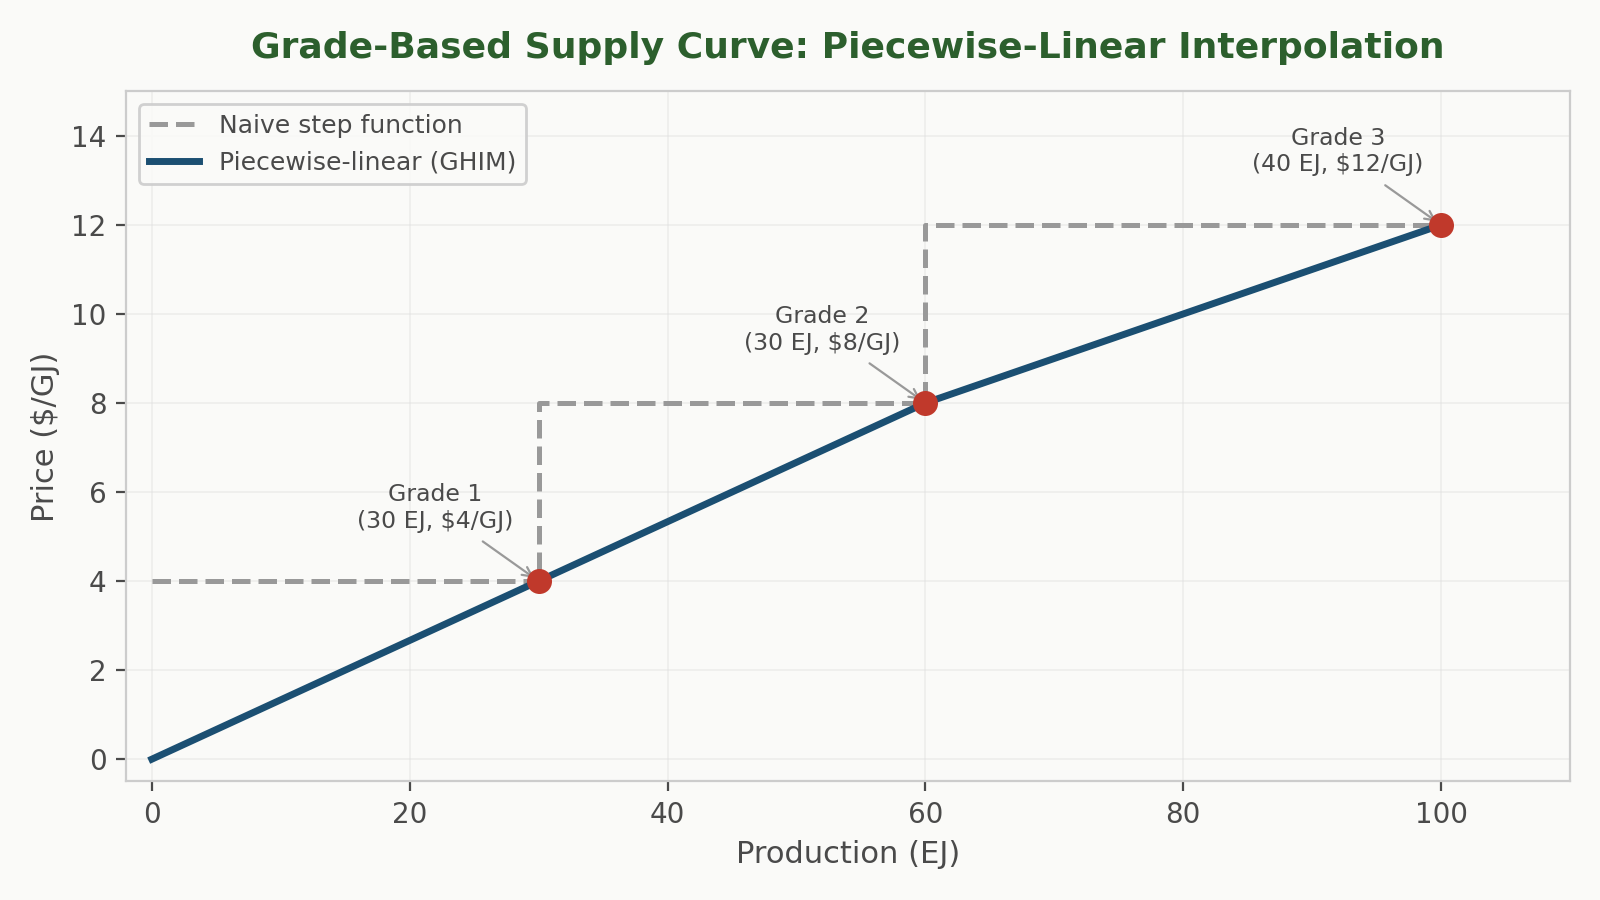
\includegraphics[width=0.50\linewidth]{supply_curve.png}
\end{center}

\end{frame}


  \begin{frame}{Primary Energy Supply --- Renewables \& Learning}

  \underline{No Resource Depletion}

  \begin{itemize}\small
    \item Wind, solar, hydro, biomass, nuclear --- supply effectively unlimited
    \item Cost determined entirely by technology capital cost (LCOE)
    \item Cost declines with cumulative deployment (learning-by-doing):
  \end{itemize}

  \vspace{0.5em}

  \begin{equation*}
    C(t) = \max\!\left(\; C_0 \cdot \left(\frac{Q_{\text{cum}}(t)}{Q_0}\right)^{\!-\beta}, \;\; 0.2 \cdot C_0 \;\right)
    \qquad \beta = \frac{\ln(1 - LR)}{\ln 2}
  \end{equation*}

  \begin{table}[ht]
  \centering
  \footnotesize
  \begin{tabular}{lcc}
  \toprule
  Technology & Learning rate\\
  \midrule
  Solar & 20\%  \\
  Wind & 12\%  \\
  Nuclear & 3\% \\
  \bottomrule
  \end{tabular}
  \end{table}

  \end{frame}

\begin{frame}{Inter-Regional Trade --- Global Market Clearing}

\begin{columns}[T]
\column{0.48\textwidth}

\underline{Global Market Clearing}
\begin{itemize}\small
  \item Single world price $p^*$ per fuel
\end{itemize}

\begin{equation*}
  \sum_r Q_r^S(p^*) = \sum_r Q_r^D(p^*)
\end{equation*}

\begin{itemize}\small
  \item Net trade: $X_r = Q_r^S - Q_r^D$
  \item $X_r>0$: exporter,\quad $X_r<0$: importer
\end{itemize}

\column{0.48\textwidth}

\underline{Implementation}
\begin{itemize}\small
  \item Fuels traded: coal, oil, gas
  \item Regions: 10 (R10)
  \item Price solved by bisection (robust)
\end{itemize}

\vspace{0.4em}
\underline{Stability}
\begin{itemize}\small
  \item Smooth price adjustment over time
\end{itemize}

\end{columns}

\end{frame}

% === Slide 1: Logit formula ===
\begin{frame}{Technology Choice}
\framesubtitle{Relative-Preference Logit}

\vspace{0.5em}

\begin{equation*}
s_i =
\frac{\alpha_i \, e^{-k P_i} \, C_i^{\beta}}
     {\sum_j \alpha_j \, e^{-k P_j} \, C_j^{\beta}}
\end{equation*}

\vspace{0.6em}

\centering
\footnotesize
\renewcommand{\arraystretch}{1.4}
\begin{tabular}{@{}ll@{}}
\toprule
Symbol & Interpretation \\
\midrule
$s_i$ & Market share of technology $i$ \\
$C_i$ & Levelized cost (\$/GJ) \\
$\beta$ & Cost sensitivity (lower cost $\Rightarrow$ higher share) \\
$P_i$ & Non-cost preference factor (\$/GJ) \\
$k$ & Preference sensitivity scale \\
$\alpha_i$ & Availability indicator (policy switch) \\
\bottomrule
\end{tabular}

\vspace{0.5em}

{\scriptsize
Combines GCAM-style relative cost choice, MERGE-style preference factors,
and explicit technology availability constraints.}

\end{frame}

\begin{frame}{Vintage Retirement}

\small
Installed capacity is tracked by technology and vintage year.

\begin{equation*}
Q_i^{\text{eff}}(t)
=
\sum_v C_{i,v} \cdot S_i(t-v)
\end{equation*}

\underline{S-curve survival (logistic)}

\begin{equation*}
S(a) = \frac{1}{1 + e^{k(a - t_{1/2})}},
\qquad
t_{1/2} = \rho \cdot L
\end{equation*}

\underline{Key assumptions}
\begin{itemize}\small
  \item Lifetime $L$ differs by technology
  \item $\rho = 0.75$: plants survive longer before rapid retirement
  \item Renewables: fixed lifetime (no S-curve)
\end{itemize}

\end{frame}

\begin{frame}{S-Curve Shutdown}
\begin{center}

    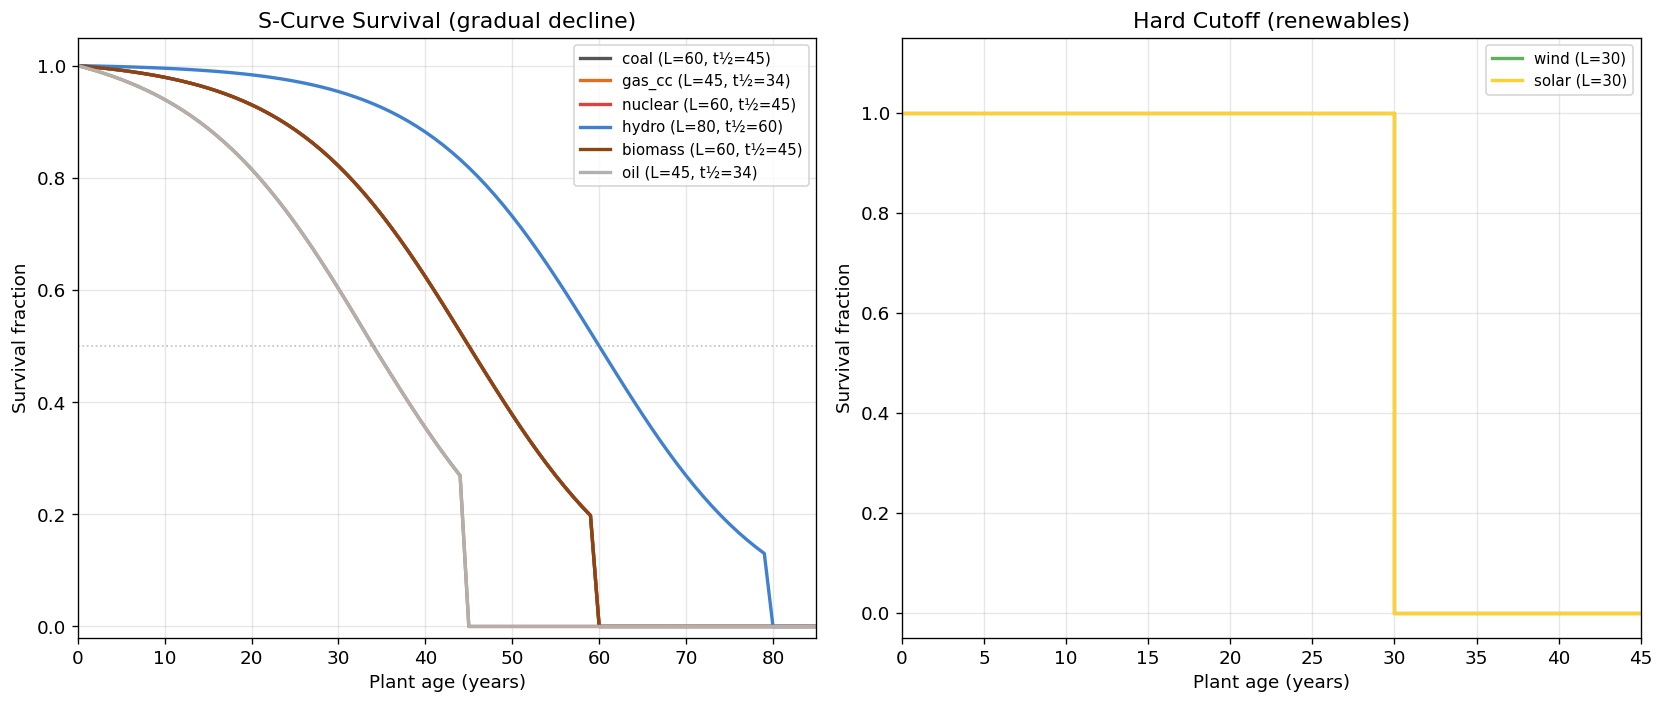
\includegraphics[width=0.85\linewidth]{scurve.png}

\end{center}
\end{frame}

\begin{frame}{Profit-Based Early Retirement}

\small
Plants may retire \textbf{before} physical end-of-life when operating losses persist.

\vspace{0.6em}

\begin{equation*}
\pi_{i,v}
=
\frac{p_{\text{elec}} - c_i^{\text{var}}}{|c_i^{\text{var}}|}
\end{equation*}

\underline{Shutdown probability}
\begin{itemize}\small
  \item Smooth S-curve in profitability
  \item Loss-making plants shut down gradually
\end{itemize}

\underline{Implication}
\begin{itemize}\small
  \item $P(\pi) \;\downarrow \quad \text{as} \quad \pi \;\downarrow$
  \item High carbon prices induce coal exit automatically
\end{itemize}

\end{frame}

\begin{frame}{Profit Shutdown}
\begin{center}

    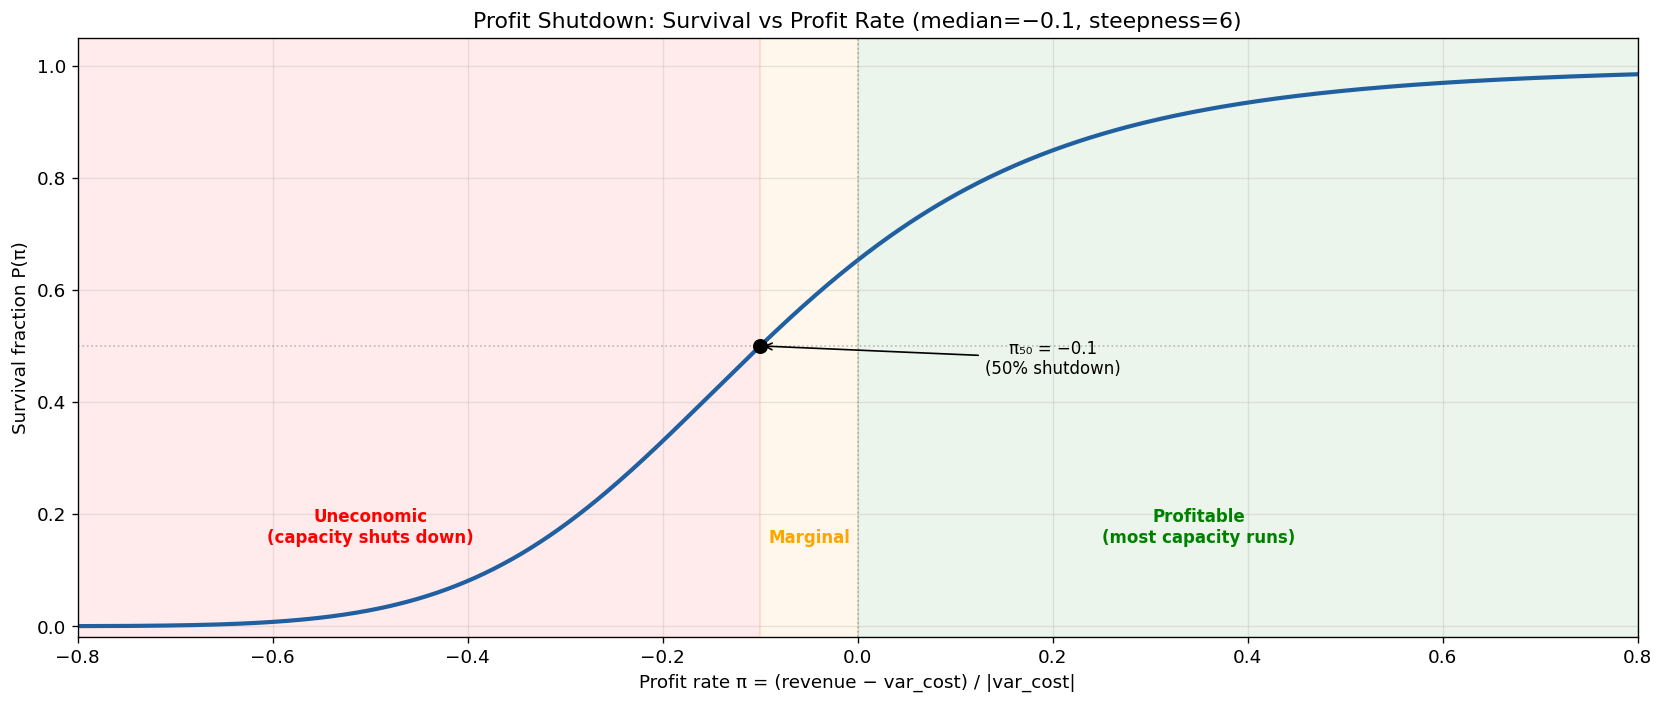
\includegraphics[width=0.85\linewidth]{profit.png}

\end{center}
\end{frame}

\begin{frame}{Construction Lead Time}

\small
New investment becomes operational only after a technology-specific build delay.

\begin{equation*}
\text{available year}
=
t + \left\lceil \frac{T_{\text{build}}}{\Delta t} \right\rceil \Delta t
\end{equation*}


\underline{Typical build times}
\begin{itemize}\small
  \item Nuclear: long lead time (one--two model periods)
  \item Large hydro: about one period
  \item Most other technologies: same-period availability
\end{itemize}

\underline{Pipeline-aware investment}
\begin{itemize}\small
  \item Capacity under construction is tracked explicitly
  \item New investment fills demand net of existing pipeline
\end{itemize}

\end{frame}


\begin{frame}{Learning-by-Doing}

\small
Investment costs decline with cumulative deployment (experience curves).

\vspace{0.6em}

\begin{equation*}
C_i(t)
=
\max\!\left[
C_{i,0}
\left(\frac{Q_i^{\text{cum}}(t)}{Q_{i,0}}\right)^{-\beta_L},
\; 0.2\,C_{i,0}
\right]
\end{equation*}


\underline{Assumptions}
\begin{itemize}\small
  \item $\beta_{L,i} = \frac{\ln(1-\text{LR}_i)}{\ln 2}$
  \item Cost floor at 20\% of initial cost
  \item No learning for mature fossil technologies
\end{itemize}

\vspace{0.6em}

\underline{Typical learning rates}
\begin{itemize}\small
  \item Solar: 20\%, Wind: 12\%, Electrolysis: 15\%
\end{itemize}


\end{frame}

\begin{frame}{Electricity Generation Mix}
\begin{center}

    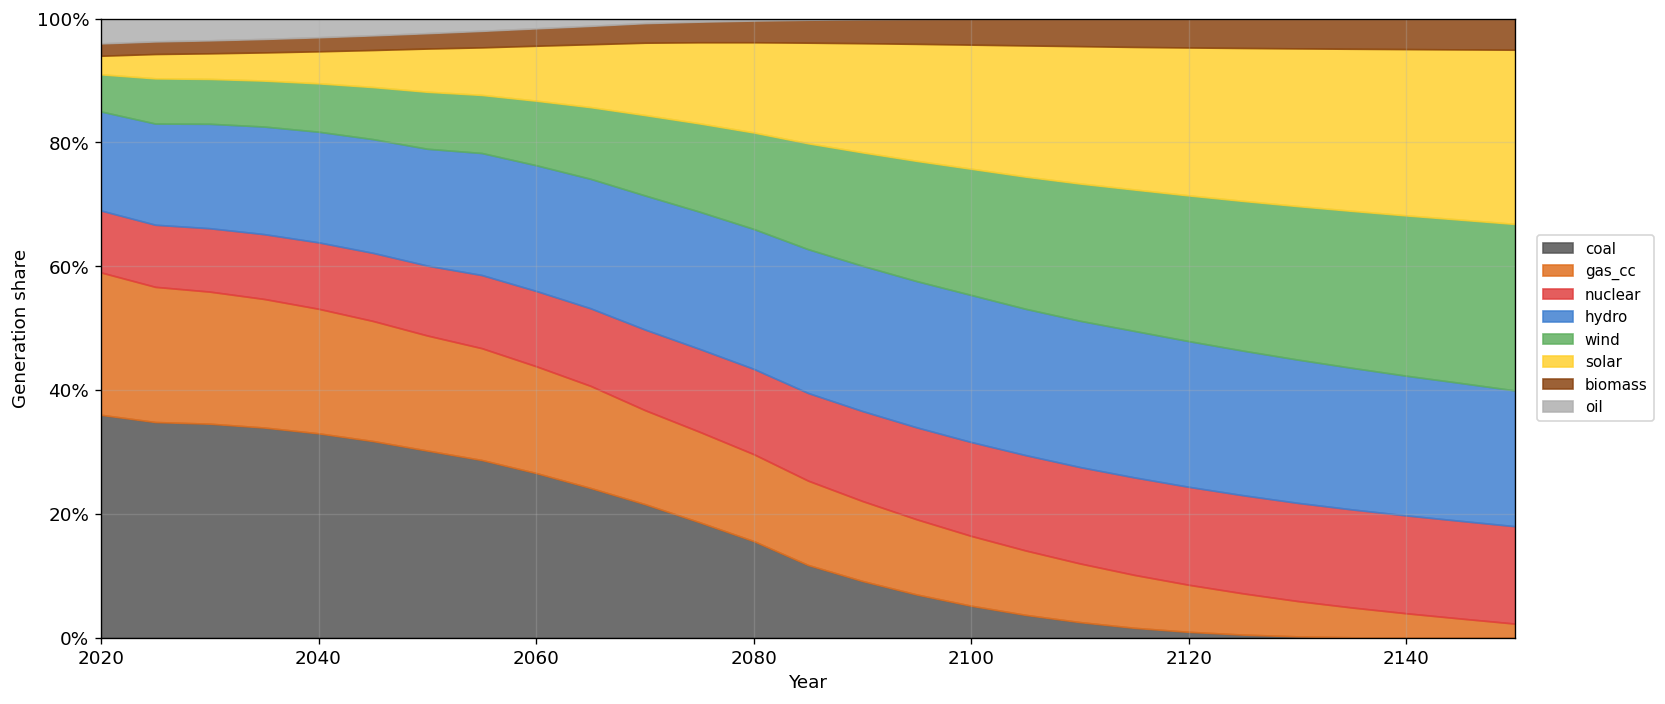
\includegraphics[width=0.85\linewidth]{elecGen.png}

\end{center}
\end{frame}

\begin{frame}{Remaining Work}

  \textbf{Model Structure}
  \begin{itemize}
    \item Capital layer consistency
    \item Recursive-dynamic $\to$ Rolling foresight
    \item R10 $\to$ Country disaggregation
    \item 5-year $\to$ 1-year timesteps
  \end{itemize}

  \vspace{0.6em}

  \textbf{Calibration, Validation \& Testing}
  \begin{itemize}
    \item Calibration from Empiricals
    \item Emulate SSPs in Detail
    \item IPCC Dataformat Outcomes
  \end{itemize}

  \end{frame}


  \begin{frame}{Repository}

  \begin{itemize}
    \item \url{https://github.com/hyuntaechoi634/ghim-energy-module}
    \item \url{https://hyuntaechoi634.github.io/ghim-energy-module}
  \end{itemize}

  \end{frame}

\end{document}
